% Fixture G8: mui ten chay doc vien khung bao.
%
% Ca 1 + 2 la LOI: duong di ap sat vien khung nhom (\node[fit=...] voi thu vien
% backgrounds), nen mat nguoi khong tach duoc dau la ranh gioi nhom, dau la
% quan he.
%
% Ca 3 la HOP LE va PHAI KHONG bao loi: duong di ben trong khung, cach vien du
% xa. Neu gate bao loi o day thi nguong dang qua chat.
%
% GHI CHU: ca 1 con sinh THEM mot finding G9/route-axis-jitter, va do la DUNG,
% khong phai bao oan. Node X dat o y=0.72cm nen doan (x1.west) -- (g1.north
% east) lech 1.87 do (2.3pt) ngay canh mot doan ngang CHINH XAC. Mat nguoi thay
% mot net gan-thang-ma-khong-thang, doc ra la cau tha. Lenh sua ma G9 de xuat
% (`|-`) dung cho chinh ca nay. Test khoa hanh vi nay lai de khong ai ve sau
% tuong la bug roi tat di.
\documentclass[border=6pt]{standalone}
\usepackage{tikz}
\usetikzlibrary{fit,backgrounds,positioning}
\begin{document}
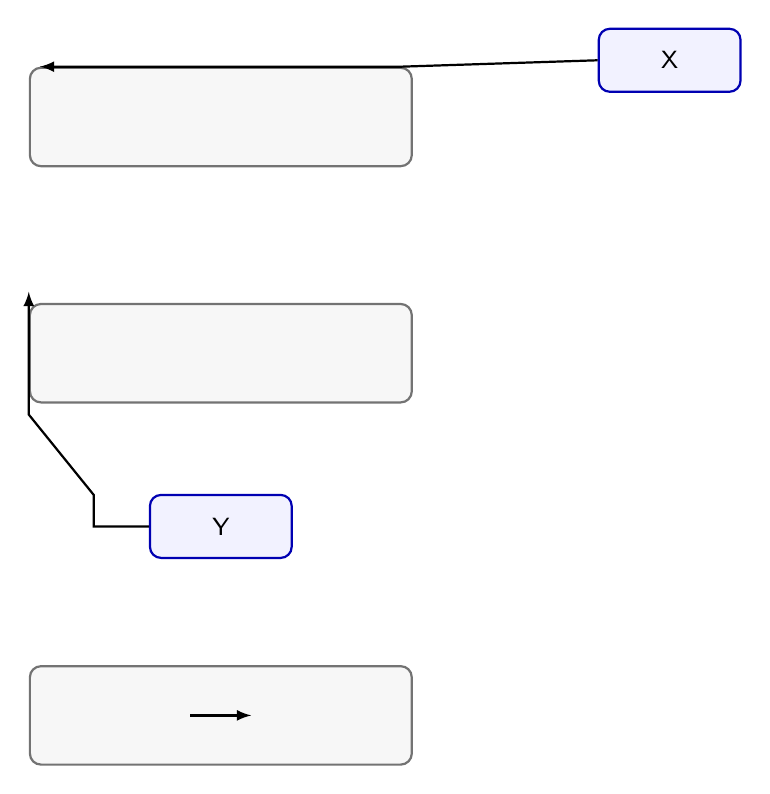
\begin{tikzpicture}[>=latex, font=\sffamily\small]
  \tikzstyle{blk}=[draw=blue!70!black, fill=blue!5, thick, rounded corners,
                   minimum width=1.8cm, minimum height=0.8cm, align=center]
  \tikzstyle{grp}=[draw=black!55, fill=black!3, thick, rounded corners,
                   inner sep=6pt]

  % ================= CA 1: chay doc vien TREN cua khung (loi) =============
  \node[blk] (a1) at (0,0)    {A};
  \node[blk] (b1) at (2.6,0)  {B};
  \node[grp, fit=(a1)(b1)] (g1) {};
  % Duong tu ngoai vao, ap sat vien tren cua g1 mot doan dai.
  \node[blk] (x1) at (7.0,0.72) {X};
  \draw[->, thick] (x1.west) -- ([xshift=-4pt]g1.north east)
                              -- ([xshift=4pt]g1.north west);

  % ================= CA 2: chay doc vien TRAI cua khung (loi) =============
  \node[blk] (a2) at (0,-3.0)   {C};
  \node[blk] (b2) at (2.6,-3.0) {D};
  \node[grp, fit=(a2)(b2)] (g2) {};
  \node[blk] (x2) at (1.3,-5.2) {Y};
  \draw[->, thick] (x2.west) -- ([xshift=-0.7cm]x2.west)
                              -- ([xshift=-0.7cm,yshift=0.4cm]x2.west)
                              -- ([yshift=-4pt]g2.south west)
                              -- ([yshift=4pt]g2.north west);

  % ============ CA 3: di BEN TRONG khung, cach vien xa (HOP LE) ===========
  \node[blk] (a3) at (0,-7.6)   {E};
  \node[blk] (b3) at (2.6,-7.6) {F};
  \node[grp, fit=(a3)(b3)] (g3) {};
  \draw[->, thick] (a3.east) -- (b3.west);
\end{tikzpicture}
\end{document}
